% Options for packages loaded elsewhere
\PassOptionsToPackage{unicode}{hyperref}
\PassOptionsToPackage{hyphens}{url}
%
\documentclass[
]{article}
\usepackage{amsmath,amssymb}
\usepackage{iftex}
\ifPDFTeX
  \usepackage[T1]{fontenc}
  \usepackage[utf8]{inputenc}
  \usepackage{textcomp} % provide euro and other symbols
\else % if luatex or xetex
  \usepackage{unicode-math} % this also loads fontspec
  \defaultfontfeatures{Scale=MatchLowercase}
  \defaultfontfeatures[\rmfamily]{Ligatures=TeX,Scale=1}
\fi
\usepackage{lmodern}
\ifPDFTeX\else
  % xetex/luatex font selection
  \setmainfont[]{Times New Roman}
  \setsansfont[]{Arial}
  \setmonofont[]{Courier New}
\fi
% Use upquote if available, for straight quotes in verbatim environments
\IfFileExists{upquote.sty}{\usepackage{upquote}}{}
\IfFileExists{microtype.sty}{% use microtype if available
  \usepackage[]{microtype}
  \UseMicrotypeSet[protrusion]{basicmath} % disable protrusion for tt fonts
}{}
\makeatletter
\@ifundefined{KOMAClassName}{% if non-KOMA class
  \IfFileExists{parskip.sty}{%
    \usepackage{parskip}
  }{% else
    \setlength{\parindent}{0pt}
    \setlength{\parskip}{6pt plus 2pt minus 1pt}}
}{% if KOMA class
  \KOMAoptions{parskip=half}}
\makeatother
\usepackage{xcolor}
\usepackage[margin=1in]{geometry}
\usepackage{graphicx}
\makeatletter
\def\maxwidth{\ifdim\Gin@nat@width>\linewidth\linewidth\else\Gin@nat@width\fi}
\def\maxheight{\ifdim\Gin@nat@height>\textheight\textheight\else\Gin@nat@height\fi}
\makeatother
% Scale images if necessary, so that they will not overflow the page
% margins by default, and it is still possible to overwrite the defaults
% using explicit options in \includegraphics[width, height, ...]{}
\setkeys{Gin}{width=\maxwidth,height=\maxheight,keepaspectratio}
% Set default figure placement to htbp
\makeatletter
\def\fps@figure{htbp}
\makeatother
\setlength{\emergencystretch}{3em} % prevent overfull lines
\providecommand{\tightlist}{%
  \setlength{\itemsep}{0pt}\setlength{\parskip}{0pt}}
\setcounter{secnumdepth}{-\maxdimen} % remove section numbering
\usepackage{booktabs}
\usepackage{caption}
\usepackage{longtable}
\usepackage{colortbl}
\usepackage{array}
\usepackage{anyfontsize}
\usepackage{multirow}
\ifLuaTeX
  \usepackage{selnolig}  % disable illegal ligatures
\fi
\usepackage{bookmark}
\IfFileExists{xurl.sty}{\usepackage{xurl}}{} % add URL line breaks if available
\urlstyle{same}
\hypersetup{
  pdftitle={2024 Job Fair Recap},
  hidelinks,
  pdfcreator={LaTeX via pandoc}}

\title{2024 Job Fair Recap}
\author{}
\date{\vspace{-2.5em}}

\begin{document}
\maketitle

\subsection{Executive Summary}\label{executive-summary}

The 2024 Job Fair series, held throughout the year, successfully
connected employers with job seekers across various industries. Key
highlights include:

Number of Employers: A total of \textbf{310} employers participated,
offering a wide range of job opportunities.

Number of Job Seekers: The series attracted \textbf{1995} job seekers,
engaging in interviews and networking with potential employers.

Job Offers Extended: \textbf{373} job offers were made during the
events, reflecting strong employer interest.

Follow-up Interviews: \textbf{1250} follow-up interviews were scheduled,
showing continued interest from employers in qualified candidates.

Overall, the 2024 Job Fair series was a highly effective platform for
connecting talent with opportunities, driving job placements and ongoing
recruitment. \[\\[1in]\]

\begin{table}[!t]
\caption*{
{\large 2024 Job Fair Recap}
} 
\fontsize{12.0pt}{14.4pt}\selectfont
\begin{tabular*}{\linewidth}{@{\extracolsep{\fill}}llllll}
\toprule
{\TEXTCOLOR[HTML]{A9A9A9}{DATE}} & {\TEXTCOLOR[HTML]{A9A9A9}{EVENT}} & {\TEXTCOLOR[HTML]{A9A9A9}{EMPLOYER}} & {\TEXTCOLOR[HTML]{A9A9A9}{JOB SEEKERS}} & {\TEXTCOLOR[HTML]{A9A9A9}{JOB OFFERS}} & {\TEXTCOLOR[HTML]{A9A9A9}{FOLLOW UP INTERVIEW}} \\ 
\midrule\addlinespace[2.5pt]
{19747} & {Health Care Career Fair} & {34} & {102} & {7} & {91} \\ 
{\bfseries \cellcolor[HTML]{rgba(70,130,180,0.8)}{\textcolor[HTML]{000000}{19843}}} & {\bfseries \cellcolor[HTML]{rgba(70,130,180,0.8)}{\textcolor[HTML]{000000}{LEDA Job Fair}}} & {\bfseries \cellcolor[HTML]{rgba(70,130,180,0.8)}{\textcolor[HTML]{000000}{128}}} & {\bfseries \cellcolor[HTML]{rgba(70,130,180,0.8)}{\textcolor[HTML]{000000}{960}}} & {\bfseries \cellcolor[HTML]{rgba(70,130,180,0.8)}{\textcolor[HTML]{000000}{232}}} & {\bfseries \cellcolor[HTML]{rgba(70,130,180,0.8)}{\textcolor[HTML]{000000}{659}}} \\ 
{19878} & {Broussard Community Job Fair} & {38} & {160} & {3} & {172} \\ 
{19928} & {2nd Chance Job Fair} & {15} & {205} & {30} & {43} \\ 
{19948} & {Industrial Trades Career Fair} & {29} & {168} & {6} & {110} \\ 
{20019} & {Acadiana Diversity Job Fair} & {66} & {400} & {95} & {175} \\ 
\bottomrule
\end{tabular*}
\end{table}

\[\\[1in]\]

\subsection{Plots}\label{plots}

\subsubsection{Employers}\label{employers}

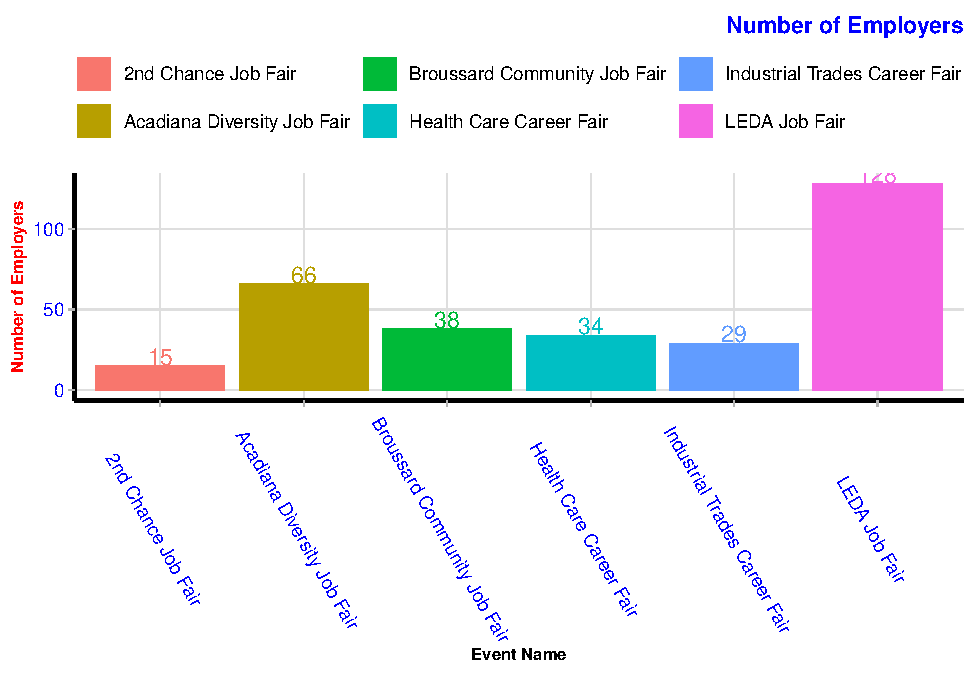
\includegraphics{2024_report_files/figure-latex/unnamed-chunk-2-1.pdf}

\subsubsection{Job Seekers}\label{job-seekers}

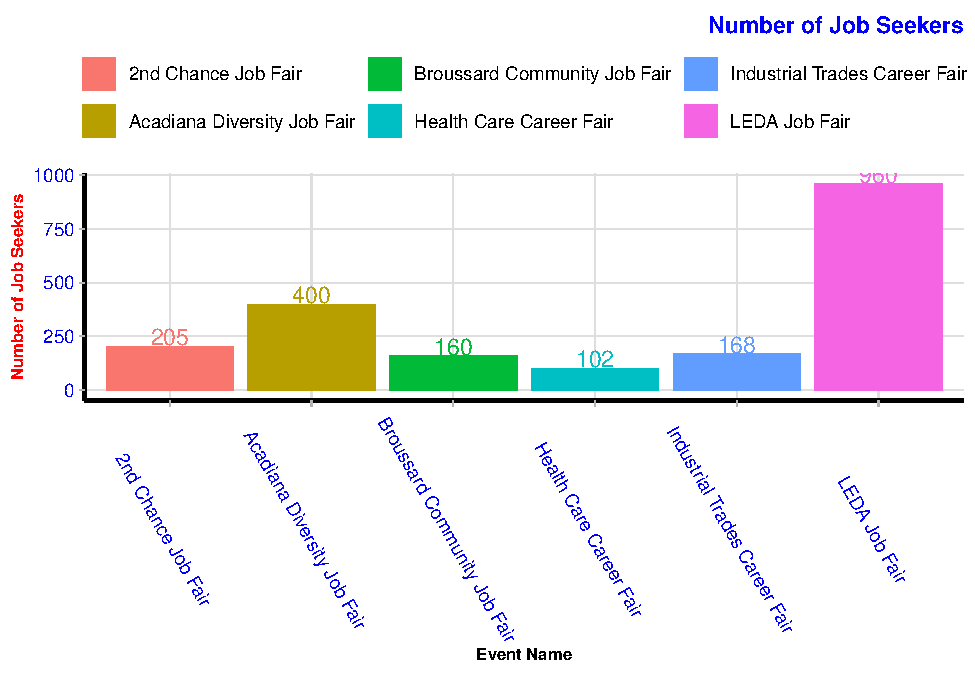
\includegraphics{2024_report_files/figure-latex/unnamed-chunk-3-1.pdf}

\subsubsection{Job Offers}\label{job-offers}

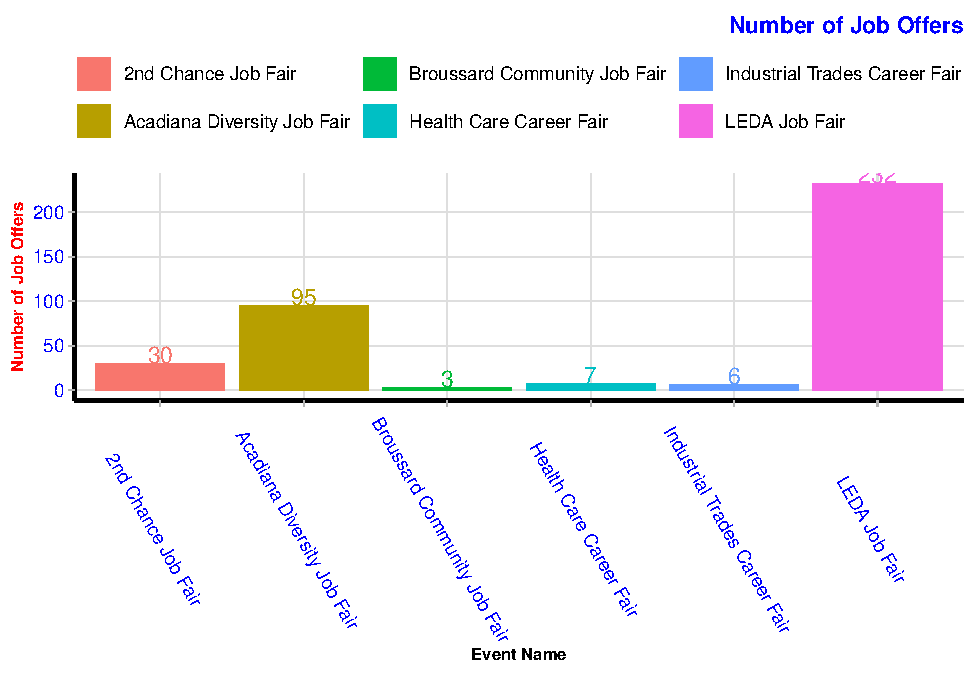
\includegraphics{2024_report_files/figure-latex/unnamed-chunk-4-1.pdf}

\subsubsection{Follow Up}\label{follow-up}

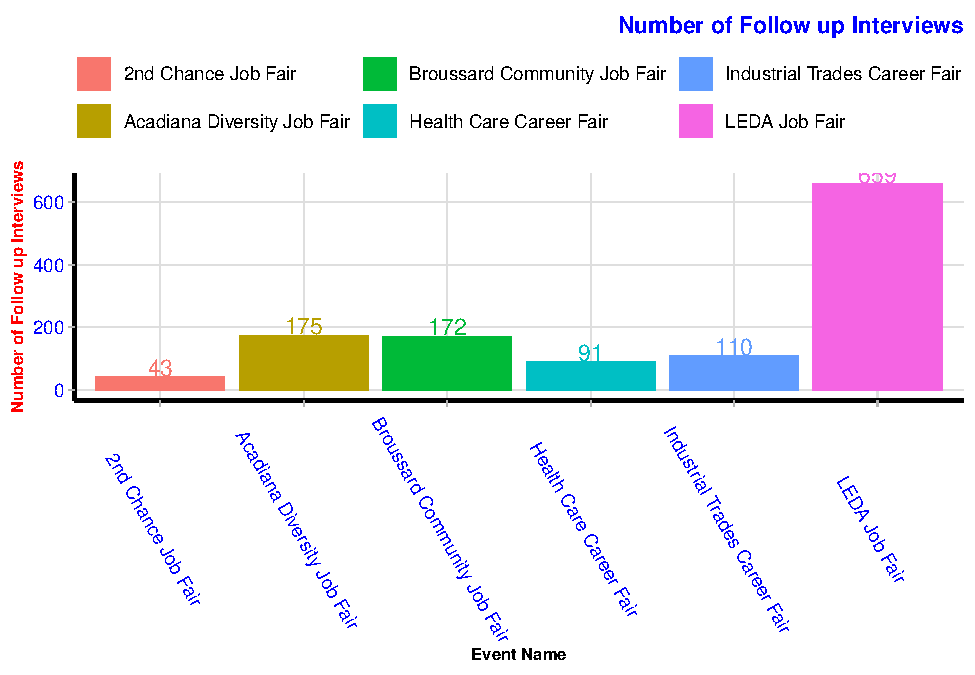
\includegraphics{2024_report_files/figure-latex/unnamed-chunk-5-1.pdf}

\end{document}
